\documentclass[main.tex]{subfiles}

\begin{document}
\subsubsection{Table no.}
Fill in your section and table number below.
\begin{itemize}
\item Section: \rule{2cm}{.15mm}
\item Table no.: \rule{2cm}{.15mm}
\end{itemize}

\subsubsection{Measurements}
Write your name, distance from object, and angular width measurement below.
\begin{table}[h!]
%\caption{default}
\begin{center}
\begin{tabular}{|p{8cm}|p{3cm}|p{3.5cm}|}\hline
Name & Distance (m) & Angular width (\si{\degree}) \\\hline
&&\\\hline
&&\\\hline
&&\\\hline
&&\\\hline
&&\\\hline
&&\\\hline
&&\\\hline
&&\\\hline
&&\\\hline
&&\\\hline
\end{tabular}
\end{center}
\label{tab:ang}
\end{table}
\vspace{-30pt}

\subsubsection{Plot}
Plot your results in the graph.

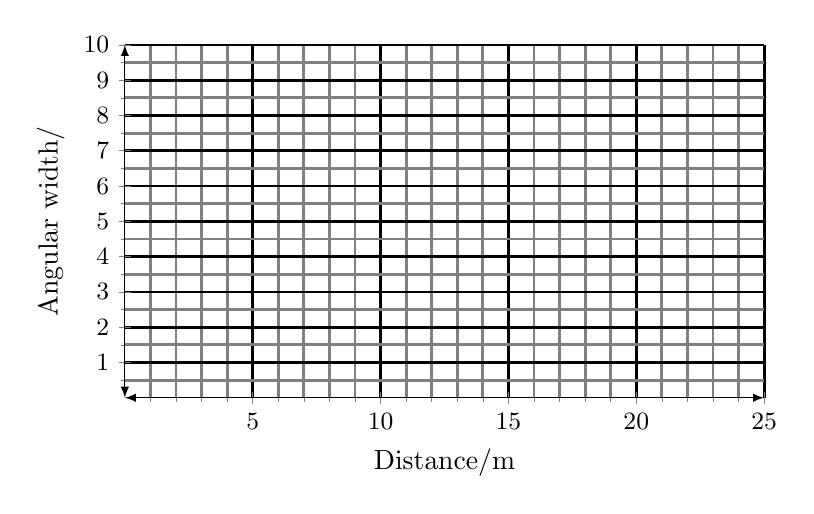
\begin{tikzpicture}
\begin{axis}[
	width=0.8\textwidth,
    height=0.5\textwidth,
    xmin=0,xmax=25,xtick={0,5,10,15,20,25},minor xtick={1,2,3,4,6,7,8,9,11,12,13,14,16,17,18,19,21,22,23,24},
    ymin=0,ymax=10,ytick={0,1,2,3,4,5,6,7,8,9,10},minor ytick={0.5,1.5,2.5,3.5,4.5,5.5,6.5,7.5,8.5,9.5},
    grid=both,
    grid style={line width=1pt, draw=gray!100},
    major grid style={line width=1pt, draw=black!100},
    axis lines=center,
    minor tick num=1,
    %enlargelimits={abs=0.5},
    axis line style={latex-latex},
    ticklabel style={font=\small},
    xlabel near ticks,
    ylabel near ticks,
    xlabel={Distance/m},
    ylabel={Angular width/\si{\degree}}
]
\end{axis}
\end{tikzpicture}

\subsubsection{Location diagram}
Mark the locations where you took your measurements in the diagram.

\begin{adjustbox}{angle=90,center,nofloat=figure}
\includegraphics[height=0.95\textwidth]{room_layout.jpg}
\end{adjustbox}

\end{document}